\section{Introduction}
In the field of autonomous mobile robotics, Simultaneous Localization And Mapping (SLAM) represents
one of the most significant problems. As the name suggests, the goal of SLAM is incrementally obtain 
from a mobile robot a map of the environment and simultaneously locate the robot's position inside it.
The difficulty of the SLAM problem is that, to precisely localize itself, the robot needs an accurate map,
of the working environment, while to obtain an accurate map, it needs an accurate localization inside the
map. This type of problems is called chicken-and-egg problem.

To get the map, SLAM algorithms take as input the observations generated by a laser sensor, typically a LiDAR, and
the odometry data from the robot's motion sensors. The laser sensor gives distance measurements and angles to
obstacles in the environment, allowing the robot to perceive its surroundings, while odometry supplies information
about the robot's movement, such as changes in position and orientation over time. By combining these two sources
of data, SLAM algorithms can incrementally build a map and estimate the robot's trajectory, even in previously 
unknown environments.

\subsection{SLAM methods}
In the last 30 years, several approaches have been developed to solve the 2D SLAM problem leading to methods 
extensively used in both common and industrial scenarios. The main paradigms \cite{Stachniss2016} used are:
\begin{itemize}
    \item Extended Kalman Filter: a vector containing the estimates of the robot position and the environment 
    landmark is used. In addition, a matrix composed of the correlations between the positions and landmark
    estimates is also used. Both the vector and the matrix are updated using the extended Kalman Filter.
    \item Particle Filter: a random sample is called a particle and it's composed of the robot position and a map
    estimate. Monte Carlo method is used to sample the possible states of the robot. The main 
    steps are: predict the robot’s pose for each particle, update particle weights based on sensor data,
    resample particles according to their weights, and update each particle’s map.
    \item Graph-based: a graph is used where nodes represent robot poses or landmarks, and edges represent
    spatial constraints derived from sensor observations or odometry. The SLAM problem is formulated as a 
    graph optimization task, where the goal is to find the configuration of nodes that best satisfies all 
    constraints, typically using nonlinear optimization techniques.
\end{itemize}

\subsection{Accuracy of SLAM methods}
The heterogeneity of SLAM methods makes it difficult to find a measure that can evaluate their performance.
Many approaches rely on manual evaluation or utilize information derived from specific algorithm.
Nowadays, the most used metric is the Absolute Pose Error (APE)\cite{APE}. The APE measures the difference over
time (Figure \ref{fig:APE}) between the estimated trajectory produced by the SLAM algorithm and the ground truth 
trajectory (Figure \ref{fig:trajectories}), focusing on the global 
consistency of the estimated poses. The big advantage of the APE is that it allows for a quantitative assessment 
of how well the SLAM algorithm reconstructs the robot's trajectory over time, independent of the internal workings 
of the specific method used.

\noindent
The APE is composed of two sub-metrics:
\begin{enumerate}
    \item The Absolute Translational Error (ATE): it measures the difference in position, typically using the 
    Euclidean distance between corresponding poses.
    \item The Absolute Rotational Error (ARE): it measures the difference in orientation, often computed as the 
    angular distance between corresponding rotations.
\end{enumerate}

\begin{figure}[htbp]
    \centering
    \begin{minipage}{0.48\textwidth}
        \centering
        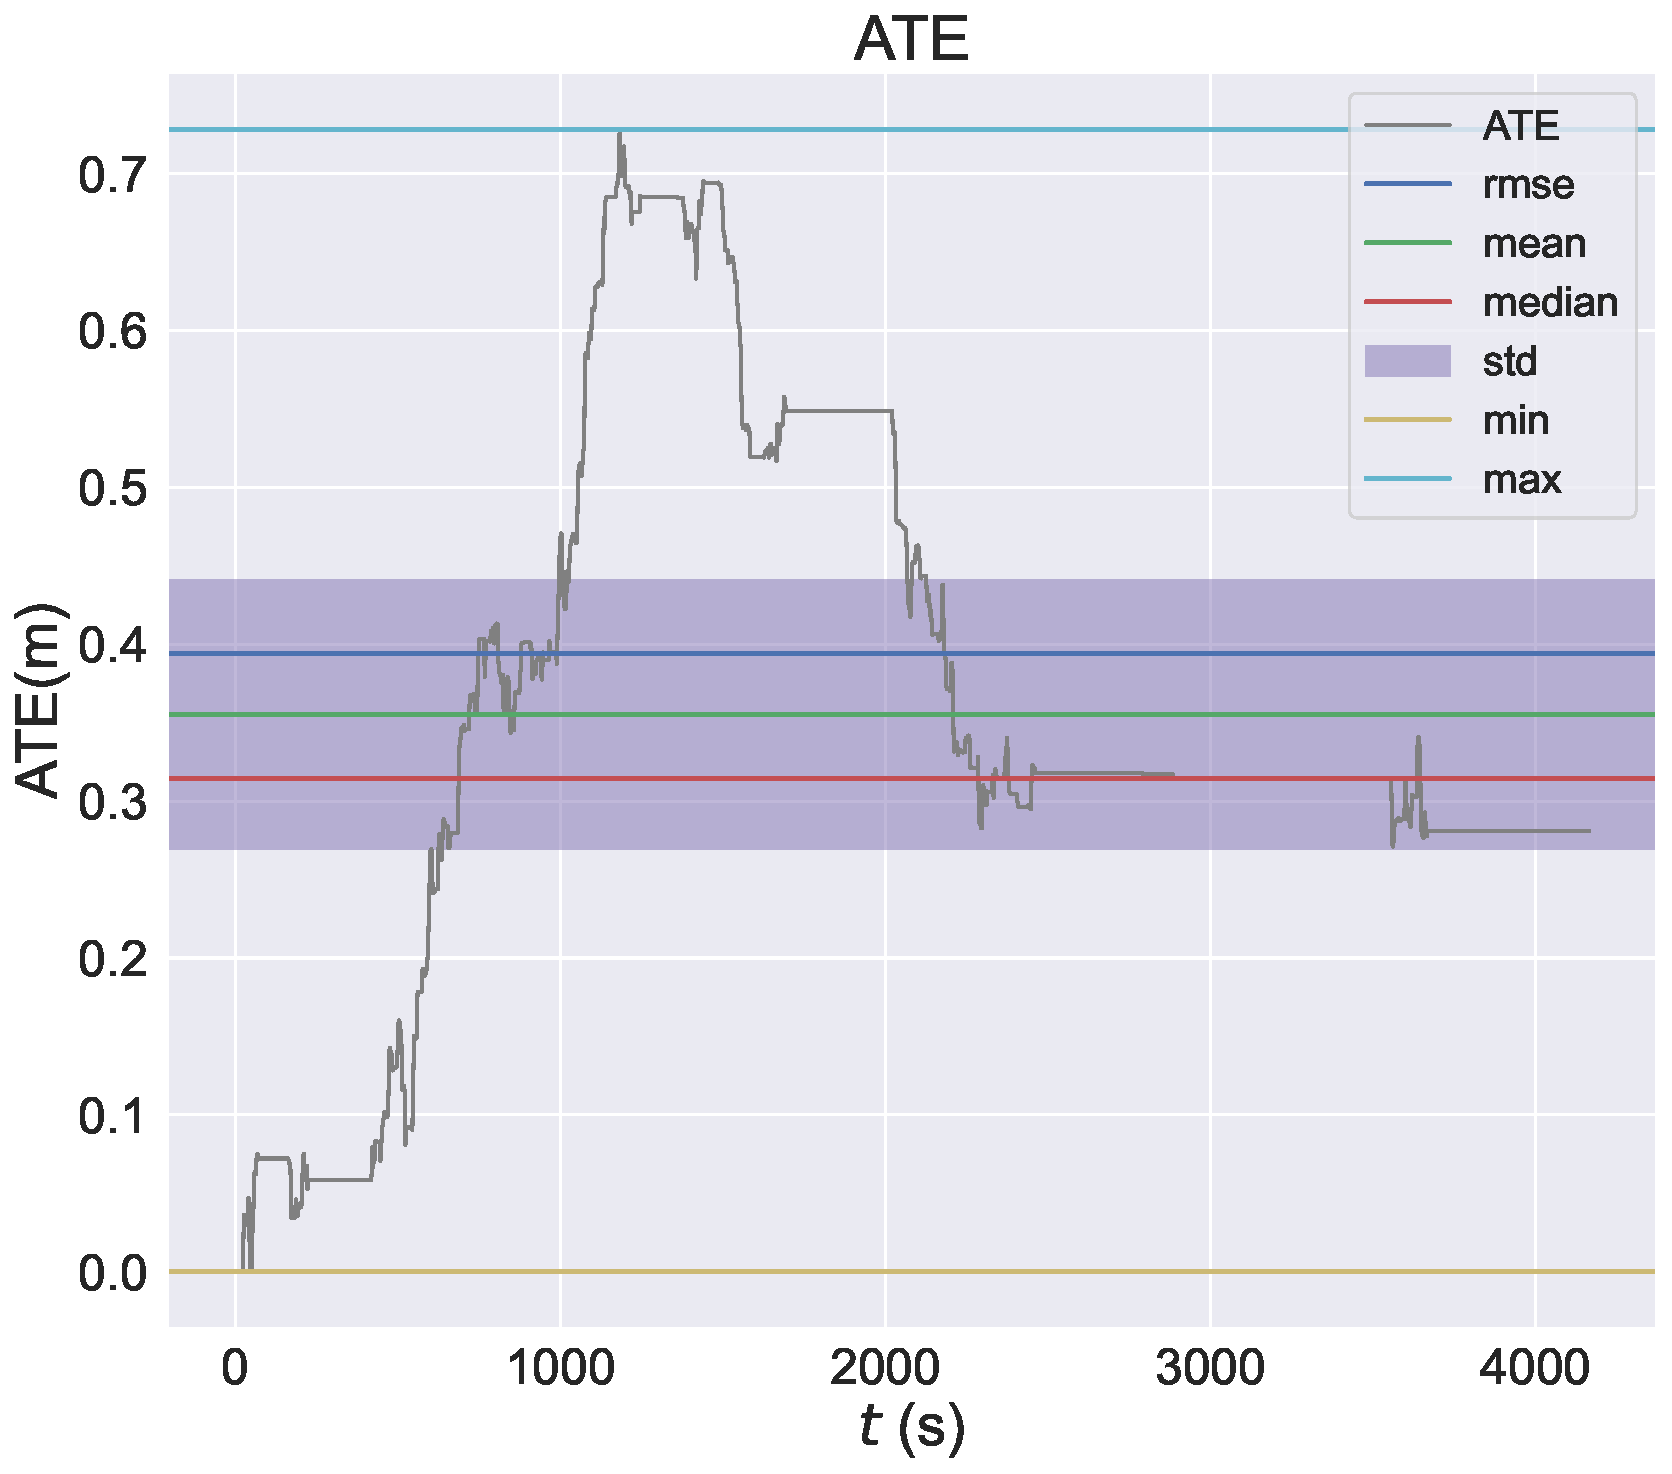
\includegraphics[width=\linewidth]{figures/APE.pdf}
        \caption{ATE variation over time during a robot mapping run shown in Figure \ref{fig:trajectories}}
        \label{fig:APE}
    \end{minipage}\hfill
    \begin{minipage}{0.48\textwidth}
        \centering
        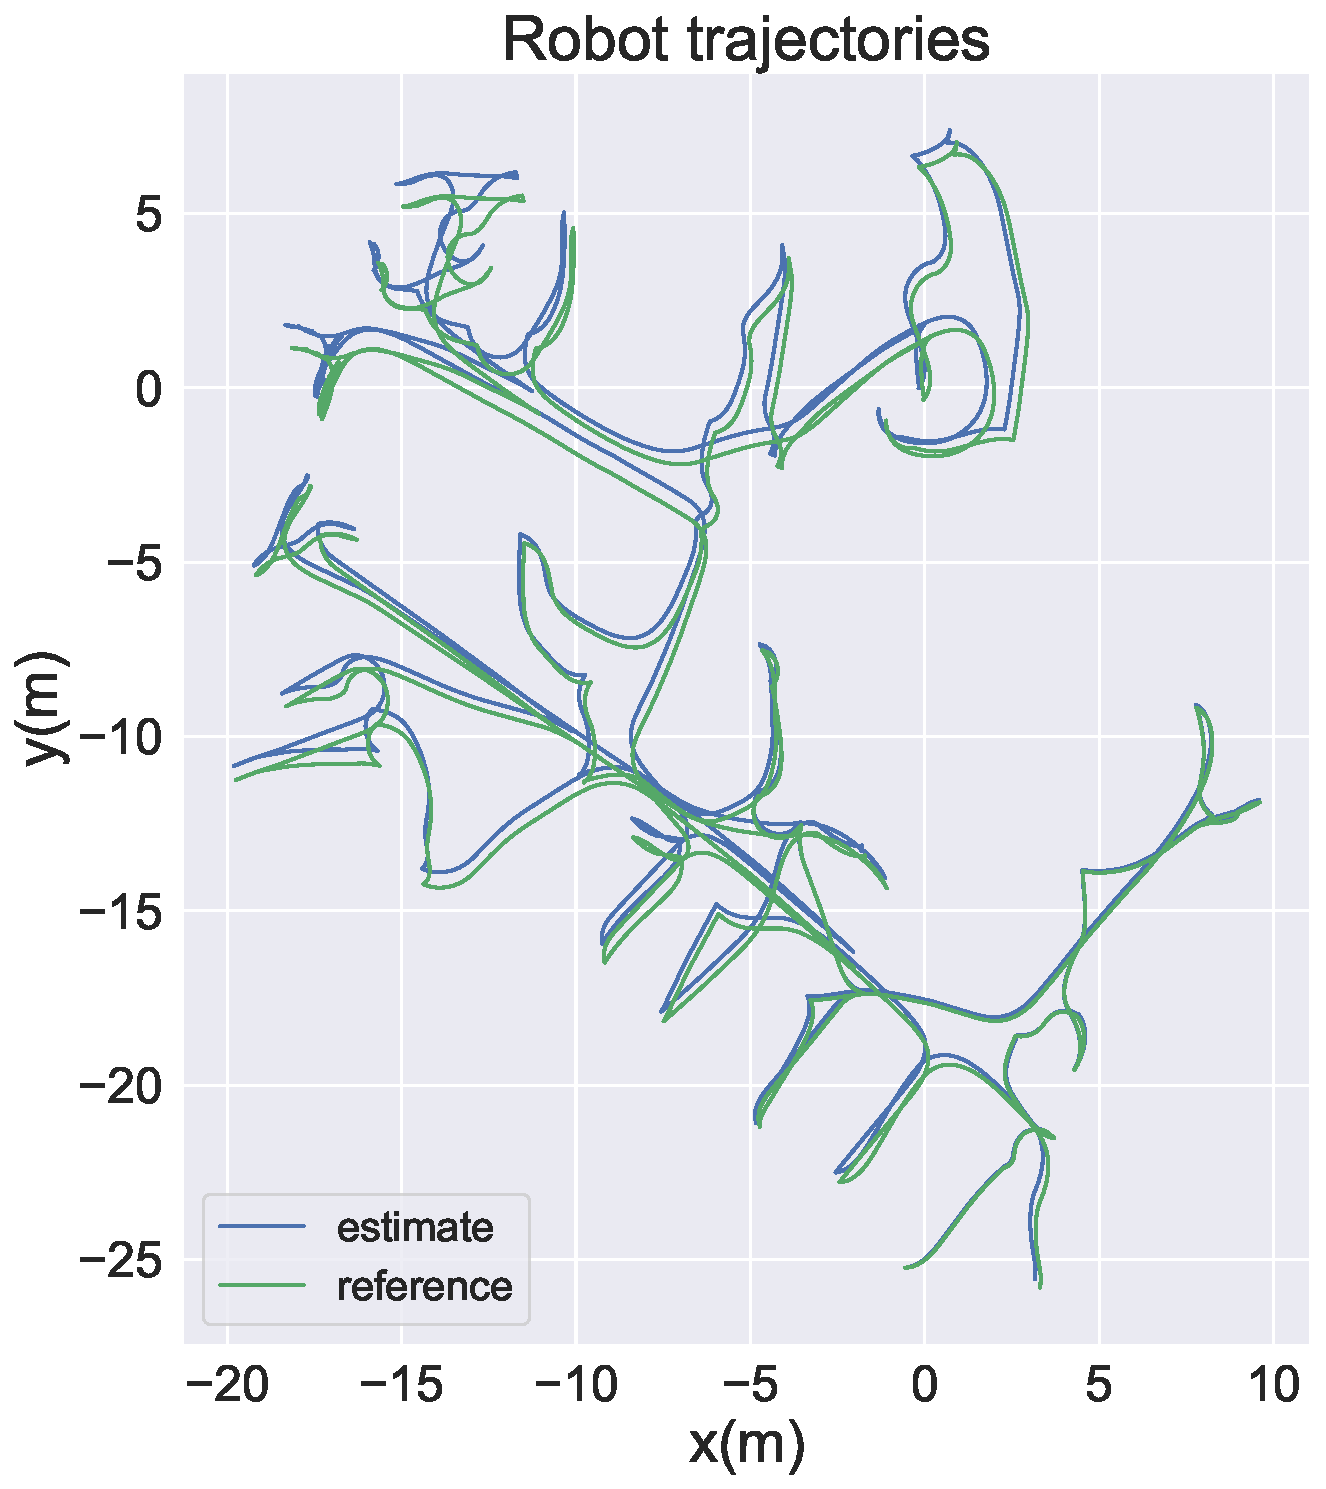
\includegraphics[width=\linewidth]{figures/trajectories.pdf}
        \caption{Difference between real (in green) and estimated (in blue) trajectory}
        \label{fig:trajectories}
    \end{minipage}
\end{figure}

\noindent
APE metric is based on the difference between the estimated robot poses and the corresponding ground truth poses. 

\noindent
Formally, let $\bm{x}_{1:T}$ be the poses of the robot estimated by
a SLAM algorithm from time step 1 to $T$, and let $\bm{x}^*_{1:T}$ be the corresponding ground truth poses.
\noindent
Let $\delta_{i,j}$ be the relative transformation that moves the robot from pose $x_i$ to $x_j$:
$$ \delta_{i,j}=x_j\ominus x_i $$
$$ \delta^*_{i,j}=x^*_j\ominus x^*_i $$ 
\noindent
Let $trans(\cdot)\in\mathbb{R}^2$ be the function that extracts the translational (position) component from a 
transformation, and let $rot(\cdot)\in\mathbb{R}^2$ extract the rotational (orientation) component as Euler angle.
\noindent
Finally, to compute the APE: 
$$
\begin{aligned}
    \displaystyle
    \text{APE} &= \underbrace{\frac{1}{N}\sum_{i,j}trans(\delta_{i,j}\ominus\delta^*_{i,j})^2}_{\text{ATE}}+
                  \underbrace{\frac{1}{N}\sum_{i,j}rot(\delta_{i,j}\ominus\delta^*_{i,j})^2}_{\text{ARE}} \\
\end{aligned}
$$

\noindent
Usually both APE and ATE and ARE are provided to assess SLAM performance.

\subsection{Project goal}
A major limitation of these metrics is their reliance on the availability of ground truth data, which is often 
difficult or impractical to obtain in real-world scenarios. Another aspect is that APE is calculated a posteriori, after the robot has explored the entire environment and so, these metrics can only be used to evaluate a run that
that has already been completed.

The main goal of this project is to propose an online estimate for the SLAM performance, specifically ATE and ARE,
in order to understand how well the robot is mapping the environment without the need to have a ground truth. This
type of prediction can be very usefull when the robot has to perform a long exploration as it allows it to recognize
an increase in the errors made by the SLAM. This type of detection allows the implementation of strategies to attempt to correct the SLAM estimates or, in the worst cases, to stop the exploration.

In this work, three different predictors will be proposed, each based on popular machine learning CNN 
architectures.
